% Solution to compiling to svg taken from 
% https://tex.stackexchange.com/a/51766
\documentclass[tikz,
	       convert={outext=.svg,command=\unexpanded{pdf2svg \infile\space\outfile}}, 	  		       multi=false]{standalone}


%\makeatletter
%\usetikzlibrary{arrows}

% Colors for diagram
\colorlet{mycolorS}{black}
\colorlet{mycolor0}{red}
\colorlet{mycolor1}{blue}
\colorlet{mycolor2}{red!20!yellow!80!}
\colorlet{mycolor3}{blue!20!green!80!}
\colorlet{mycolor4}{cyan!10!}
\colorlet{mycolor5}{yellow!10!}
\colorlet{mycolor6}{magenta!10!}
\colorlet{mycolor7}{green!10!}


\begin{document}
    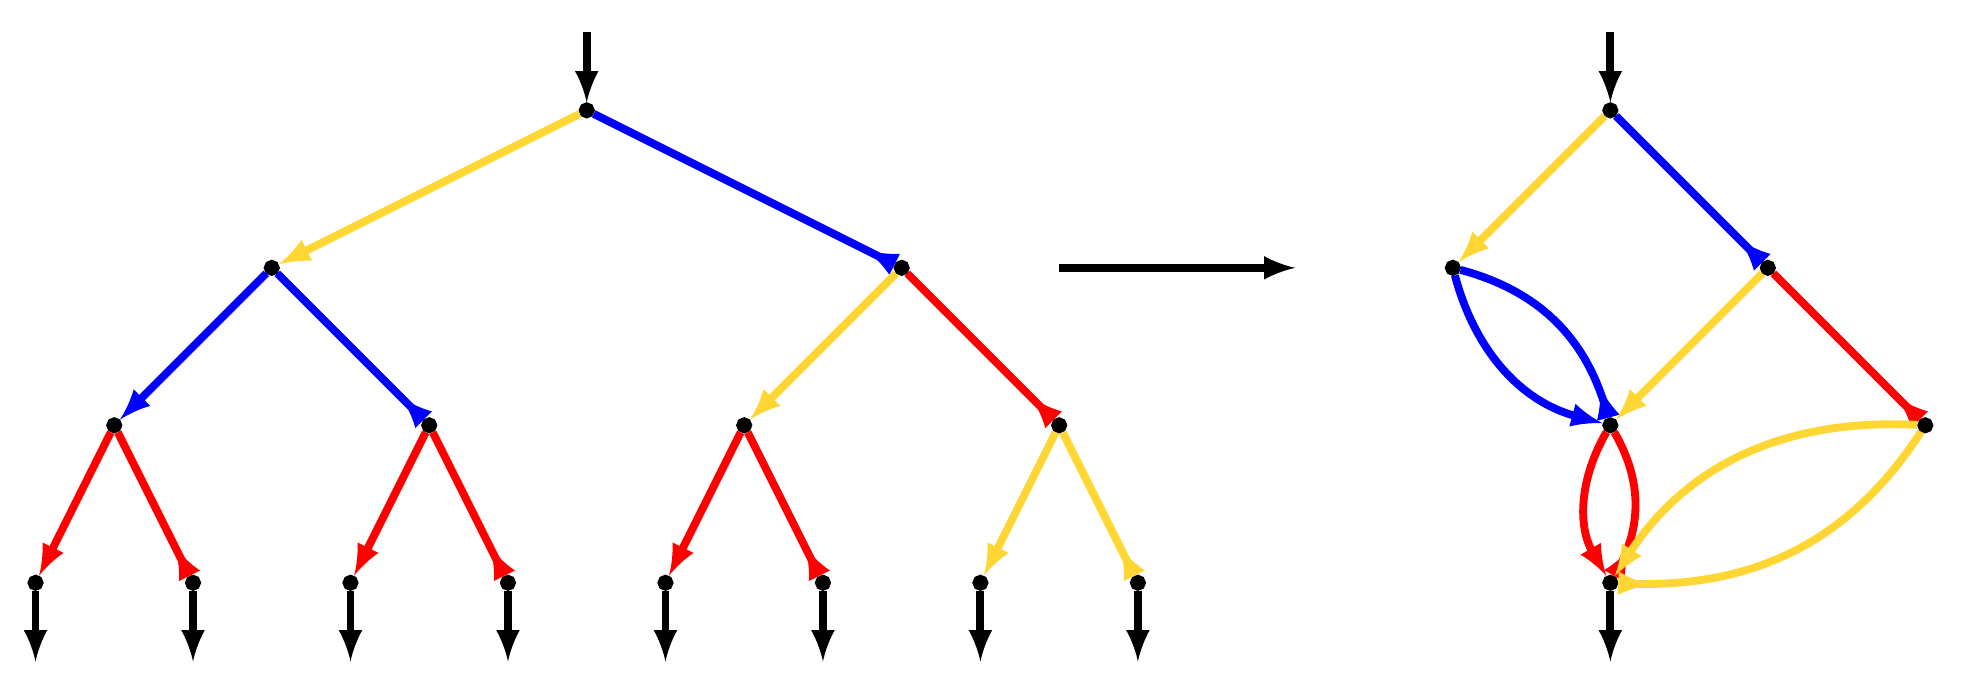
\begin{tikzpicture}[line width=1mm,
        every node/.style={circle, draw, fill=black, inner sep=0pt, minimum
        width=1mm}
        ]
        \begin{scope}[xshift=-8cm]
            \node (q_e) at (0,0) {};
            \node (q_0) at (-4, -2) {}; 
            \node (q_1) at (4, -2) {};
            \node (q_00) at (-6, -4) {};
            \node (q_01) at (-2, -4) {}; 
            \node (q_10) at (2, -4) {}; 
            \node (q_11) at (6, -4) {};
            \node (q_000) at (-7, -6) {};
            \node (q_001) at (-5, -6) {};
            \node (q_010) at (-3, -6) {};
            \node (q_011) at (-1, -6) {};
            \node (q_100) at (1, -6) {};
            \node (q_101) at (3, -6) {};
            \node (q_110) at (5, -6) {};
            \node (q_111) at (7, -6) {};
    \draw [-latex] (q_e)++(0,1) -- (q_e);
    \draw [-latex,draw=mycolor2] (q_e) -- (q_0);
    \draw [-latex reversed,draw=mycolor1] (q_e) -- (q_1);
    \draw [-latex,draw=mycolor1] (q_0) -- (q_00);
    \draw [-latex reversed,draw=mycolor1] (q_0) -- (q_01);
    \draw [-latex,draw=mycolor2] (q_1) -- (q_10);
    \draw [-latex reversed,draw=mycolor0] (q_1) -- (q_11);
    \draw [-latex,draw=mycolor0] (q_00) -- (q_000);
    \draw [-latex reversed,draw=mycolor0] (q_00) -- (q_001);
    \draw [-latex,draw=mycolor0] (q_01) -- (q_010);
    \draw [-latex reversed,draw=mycolor0] (q_01) -- (q_011);
    \draw [-latex,draw=mycolor0] (q_10) -- (q_100);
    \draw [-latex reversed,draw=mycolor0] (q_10) -- (q_101);
    \draw [-latex,draw=mycolor2] (q_11) -- (q_110);
    \draw [-latex reversed,draw=mycolor2] (q_11) -- (q_111);
    \draw [-latex] (q_000) -- ++(0,-1);
    \draw [-latex] (q_001) -- ++(0,-1);
    \draw [-latex] (q_010) -- ++(0,-1);
    \draw [-latex] (q_011) -- ++(0,-1);
    \draw [-latex] (q_100) -- ++(0,-1);
    \draw [-latex] (q_101) -- ++(0,-1);
    \draw [-latex] (q_110) -- ++(0,-1);
    \draw [-latex] (q_111) -- ++(0,-1);
\end{scope}

    
    \draw [-latex] (-2,-2) -- (1,-2);

        \begin{scope}[xshift=5cm]
            \node (q_e) at (0,0) {};
            \node (q_0) at (-2, -2) {}; 
            \node (q_1) at (2, -2) {};
            \node (q_10) at (0, -4) {}; 
            \node (q_11) at (4, -4) {};
            \node (q_000) at (0, -6) {};
    \draw [-latex] (q_e)++(0,1) -- (q_e);
    \draw [-latex,draw=mycolor2] (q_e) -- (q_0);
    \draw [-latex reversed,draw=mycolor1] (q_e) -- (q_1);
    \draw [-latex,draw=mycolor1, ] (q_0) to[out=-75,in=165] (q_10);
    \draw [-latex reversed,draw=mycolor1] (q_0) to[out=-15,in=105] (q_10);
    \draw [-latex,draw=mycolor2] (q_1) -- (q_10);
    \draw [-latex reversed,draw=mycolor0] (q_1) -- (q_11);
    \draw [-latex,draw=mycolor0] (q_10) to[out=-120, in=120] (q_000);
    \draw [-latex reversed,draw=mycolor0] (q_10) to[out=-60, in=60](q_000);
    \draw [-latex,draw=mycolor2] (q_11) to[out=-183,in=57] (q_000);
    \draw [-latex reversed,draw=mycolor2] (q_11) to[out=-123, in=-3] (q_000);
    \draw [-latex] (q_000) -- ++(0,-1);
\end{scope}
\end{tikzpicture}
\end{document}

